%% LaTeX Beamer presentation template (requires beamer package)
%% see http://latex-beamer.sourceforge.net/
%% idea contributed by H. Turgut Uyar
%% template based on a template by Till Tantau
%% this template is still evolving - it might differ in future releases!

\documentclass[hyperref={pdfpagelabels=false}]{beamer}

\mode<presentation>

% $Id: macros.tex,v 1.4 2013/08/18 16:00:29 ganeshau Exp $
%\usepackage[pdftex]{hyperref}
\frenchspacing
\usepackage{mathptmx}

%\usepackage{cite}
\usepackage[T1]{fontenc}
\usepackage{times}
\usepackage{url}
%\usepackage{cite}
\usepackage{amsmath}
% \usepackage{fancyhdr}
%\usepackage{fancyvrb}
%\usepackage{fancybox}
\usepackage{color}
\usepackage{colortbl}
\usepackage{mathpartir}
\usepackage{amssymb}
\usepackage{xspace}
\usepackage{comment}
\usepackage{graphicx}
\graphicspath{{figures/}}
%\usepackage{epsfig}
%\usepackage{wrapfig}
\usepackage{multirow}
%\usepackage{subfig}

% Added listing for code listings
\usepackage{listings}
\usepackage{relsize}
%\usepackage{stfloats}
\usepackage{fixltx2e}
\usepackage{courier}
% formatting for grammars
% \input{obey}
% \input{grammar}

\usepackage{soul}
\newcommand{\hlc}[2][yellow]{ {\sethlcolor{#1} \hl{#2}} }

%\renewcommand{\nonterm}[1]{\mbox{\textit{#1}}}
\newcommand{\oneormore}[1]{#1\ensuremath{^+}}

% % %\newcommand{\panini}{\textsf{java}$_c$\xspace}
% \newcommand{\mechanism}{active module\xspace}
% \newcommand{\Mechanism}{Active module\xspace}
% \newcommand{\MEchanism}{Active Module\xspace}
% \newcommand{\mechanisms}{active modules\xspace}
% \newcommand{\Mechanisms}{Active modules\xspace}
% \newcommand{\MEchanisms}{Active Modules\xspace}
%\newcommand{\intermechanism}{inter-modular\xspace}
%\newcommand{\intramechanism}{intra-modular\xspace}

\newcommand{\mechanism}{capsule\xspace}
\newcommand{\Mechanism}{Capsule\xspace}
\newcommand{\MEchanism}{Calsupe\xspace}
\newcommand{\mechanisms}{capsules\xspace}
\newcommand{\Mechanisms}{Capsules\xspace}
\newcommand{\MEchanisms}{Capsules\xspace}
\newcommand{\intermechanism}{inter-capsular\xspace}
\newcommand{\intramechanism}{intra-capsular\xspace}

\newcommand{\MRB}{Message Ring Buffer\xspace}
\newcommand{\mrb}{message ring buffer\xspace}
\newcommand{\TaskFramework}{task framework\xspace}

% Type checking macros
% change symbol type of : from mathrel 
%\DeclareMathSymbol{:}{\mathbin}{operators}{"3A} 
\newcommand{\OK}{\mbox{OK}}
\newcommand{\OKin}{\mbox{OK in }}
\newcommand{\inC}{\mbox{in }c}
\newcommand{\isType}{\mbox{\textit{isType}}}
\newcommand{\validFields}{\mbox{\textit{validF}}}
\newcommand{\isClass}{\mbox{\textit{isClass}}}
\newcommand{\isHandler}{\mbox{\textit{isHandler}}}
\newcommand{\Types}{\mbox{\textit{Types}}}
\newcommand{\Names}{\mbox{\textit{Names}}}
\newcommand{\TypeEnv}{\mbox{\textit{TypeEnv}}}
\newcommand*{\findMeth}{\auxFunc{findMeth}}
\newcommand*{\fieldsOf}{\auxFunc{fields}}
\newcommand*{\fieldName}{\auxFunc{fieldName}}
\newcommand*{\checkMethods}{\auxFunc{methE}}
\newcommand*{\methodEffect}{\auxFunc{me}}
\newcommand*{\typeOfField}{\auxFunc{typeOfF}}
\newcommand*{\typeOf}{\auxFunc{typeOf}}
\newcommand*{\dom}{\auxFunc{dom}}
\newcommand*{\rng}{\auxFunc{rng}}
\newcommand*{\isAnn}{\auxFunc{annotated}}
\newcommand*{\updateEffect}{\auxFunc{update}}
\newcommand*{\reversePointer}{\auxFunc{reverse}}
\newcommand*{\reversePoint}{\auxFunc{reverseP}}
\newcommand*{\fixPoint}{\auxFunc{fixPoint}}
\newcommand*{\updateOther}{\auxFunc{updateOther}}
\newcommand*{\updateMethodEffect}{\auxFunc{updateEff}}
\newcommand*{\updateSingleMethodEffect}{\auxFunc{updateMeth}}
\newcommand*{\updateSingleEffect}{\auxFunc{concretize}}
\newcommand*{\updateForkEffect}{\auxFunc{updateFork}}
\newcommand*{\updateQueue}{\auxFunc{updateQ}}
\newcommand*{\getActive}{\auxFunc{active}\xspace}
\newcommand*{\field}{\auxFunc{field}}
\newcommand{\fdecl}{\mbox{\textit{fdecl}}}
\newcommand*{\fieldOf}{\auxFunc{fieldOf}}
\newcommand*{\getOpen}{\auxFunc{getOpen}}
\newcommand{\NPE}{\mbox{\textit{NPE}}}

% Reserved words (in math mode)
\newcommand{\Extends}{\mbox{\texttt{\textbf{extends}}}}
\newcommand{\Implements}{\mbox{\texttt{\textbf{implements}}}}
\newcommand{\This}{\mbox{\texttt{\textbf{this}}}}
\newcommand{\Self}{\mbox{\texttt{\textbf{self}}}}
\newcommand{\EV}{\mbox{\texttt{\textbf{event}}~}}
\newcommand{\Cast}{\mbox{\texttt{\textbf{cast}}}}
\newcommand{\New}{\mbox{\texttt{\textbf{new}}~}}
\newcommand{\Null}{\mbox{\texttt{\textbf{null}}}}
\newcommand{\Chain}{\mbox{\texttt{\textbf{chain}}~}}
\newcommand{\Under}{\mbox{\texttt{\textbf{under}}~}}
\newcommand{\If}{\mbox{\texttt{\textbf{if}}}}
\newcommand{\Then}{\mbox{\texttt{\textbf{then}}}}
\newcommand{\Else}{\mbox{\texttt{\textbf{else}}}}
\newcommand{\While}{\mbox{\texttt{\textbf{while}}}}

% Aux functions
\newcommand{\auxFunc}[1]{\ensuremath{\mathop{\mathit{#1}}}}
\newcommand*{\override}{\auxFunc{override}}

% types
\newcommand{\POWERSET}[1]{\mbox{\textit{PowerSet}}(#1)}
\newcommand{\delete}{\mbox{\textit{delete}}}
\newcommand{\mklist}{\mbox{\textit{mksupers}}}
\newcommand{\uminus}{\mbox{$\cup\!\!\!\!-$}}
\newcommand{\iminus}{\mbox{$\cap\!\!\!\!-$}}
\newcommand{\commutesWith}{\sharp}
\newcommand{\notCommutesWith}{\not\sharp}
\newcommand{\rname}[1]{$\TirName{(#1)}$} % for inline inferrule names
\newcommand{\STO}{\ensuremath{<:}}  % ``subtype of''
\newcommand{\notSTO}{\ensuremath{\not<:}}  % ``subtype of''
\newcommand{\consistent}{\ensuremath{\approx}}

% auxiliary funtions for finding the dynamic effects for program executions.
\newcommand*{\dynamicInfinite}{\auxFunc{dynValue}}
\newcommand*{\dynamicEffects}{\auxFunc{dynE}}
\newcommand*{\dynamicEffectsOnce}{\auxFunc{dyn}}
\newcommand*{\dynamicEffectSet}{\auxFunc{dynESet}}
\newcommand*{\predecessorSiblings}{\auxFunc{preS}}
\newcommand*{\predSibles}{\auxFunc{pSib}}
%\newcommand*{\offspring}{\auxFunc{descendentsOf}}
%\newcommand*{\offspring}{\auxFunc{descendents}}
\newcommand*{\offspring}{\auxFunc{desc}}
\newcommand*{\offspringOrItself}{\auxFunc{descendOrSelf}} 
\newcommand*{\inQueueX}{\auxFunc{inQ}} 
\newcommand*{\inQueueY}{\auxFunc{inq}}
\newcommand*{\replaceQueue}{\auxFunc{replace}}
\newcommand*{\substituteSequence}{\auxFunc{subSeq}}
\newcommand*{\combineSequence}{\auxFunc{comSeq}}
\newcommand*{\mergeSequence}{\auxFunc{merSeq}}
\newcommand*{\isin}{\auxFunc{belongs}}
\newcommand*{\configuration}{c}

% Macros for operational semantics
\newcommand{\mc}[1]{\mbox{\rm \ensuremath{\text{\code{#1}}}}} % Arg set in code font in math
\newcommand{\loc}{\ensuremath{\mathord{\mathit{loc}}}}
\newcommand{\handler}[3]{\ensuremath{\langle#1,#2,#3\rangle}}
\newcommand{\ec}{\ensuremath{\mathbb{E}}}
%\newcommand{\ec}{\ensuremath{\mathop{\mathbb{E}}}}
%\newcommand{\ecpending}{\ensuremath{\mathop{\mathbb{E'}}}}
\newcommand{\ecpending}{\ensuremath{\mathop{\overline{\mathbb{E}}}}}
\newcommand{\hole}{\ensuremath{\mathord{\mathit{-}}}}
\newcommand{\reducesto}{\hookrightarrow}
\newcommand{\reducestostar}{\overset{*}{\reducesto}}
\newcommand{\dontcare}{\ensuremath{\mathord{\text{\textvisiblespace\hspace{0.10ex}}}}}
\newcommand{\Expression}{\ensuremath{{\cal E}}}
\newcommand{\Stack}{\mbox{\textit{Stack}}}
\newcommand{\Store}{\mbox{\textit{Store}}}
\newcommand{\ActiveList}{\mbox{\textit{ActiveList}}}
\newcommand{\Frame}{\mbox{\textit{Frame}}}
\newcommand{\FieldEnv}{\mbox{\textit{FieldEnv}}}
\newcommand{\ObjectRecord}{\mbox{\textit{ObjectRecord}}}
\newcommand{\lexframe}{\mbox{\textbf{\texttt{frame}}}}
\newcommand{\handlerframe}{\mbox{\textbf{\texttt{hframe}}}}
\newcommand{\Excep}{\mbox{\textit{Excep}}}

\newcommand*{\seq}[1]{\ensuremath{\left\langle {#1} \right\rangle}} % Arg is sequence contents
\newcommand{\config}{\seq}
\newcommand{\udot}{\mathbin{\sqcup \kern-0.53em \cdot \,}}

\newcommand{\eseq}{\hat{e}}

% Effect attributes
\newcommand{\ReadE}{\mbox{\texttt{\textbf{read}}~}}
%\newcommand{\WriteE}{\mbox{\texttt{\textbf{write}}~}}
\newcommand{\WriteE}{\mbox{\texttt{\textbf{write}}~}}
\newcommand{\CheckE}{\mbox{\texttt{\textbf{open}}}}
%\newcommand{\ForkE}{\mbox{\texttt{\textbf{fork}}}}
\newcommand{\ForkE}{\mbox{\texttt{\textbf{fork}}}}
\newcommand{\EnqueueE}{\mbox{\texttt{\textbf{bottom}}}}
%\newcommand{\BottomE}{\mbox{\texttt{\textbf{\bot}}}}
\newcommand{\RegisterE}{\mbox{\texttt{\textbf{exp}}}}
%\newcommand{\AnnounceE}{\mbox{\texttt{\textbf{frk}}~}}
\newcommand{\CreateE}{\mbox{\texttt{\textbf{create}}~}}
% Effect Auxiliary Functions
\newcommand*{\EffectsOf}{\auxFunc{effects}}
\newcommand{\ReadF}{\mbox{\texttt{\textbf{rd}}}}
\newcommand{\WriteF}{\mbox{\texttt{\textbf{wt}}}}
\newcommand{\ForkF}{\mbox{\texttt{\textbf{fk}}}}
\newcommand{\EnqueueF}{\mbox{\texttt{\textbf{eq}}}}
\newcommand{\BottomF}{\mbox{\texttt{\textbf{bt}}}}
\newcommand{\ConcretizedF}{\mbox{\texttt{\textbf{ct}}}}
\newcommand{\OtherF}{\mbox{\texttt{\textbf{el}}}}


\newcommand{\Class}{\mbox{\texttt{\textbf{class}}~}}
\newcommand{\tasks}{\mbox{\texttt{\textbf{tasks}}~}}
\newcommand{\fork}{\mbox{\texttt{\textbf{fork}}~}}
\newcommand{\foreach}{\mbox{\texttt{\textbf{forall}}~}}
\newcommand{\Decl}{\mbox{\texttt{\textbf{decl}}~}}
\newcommand{\RDecl}{\mbox{\texttt{\textbf{rdecl}}~}}
\newcommand{\Exp}{\mbox{\texttt{\textbf{exp}}~}}
\newcommand{\Prog}{\mbox{\texttt{\textbf{prog}}~}}
\newcommand{\Meth}{\mbox{\texttt{\textbf{meth}}~}}
\newcommand{\Type}{\mbox{\texttt{\textbf{type}}}}
\newcommand{\var}{\mbox{\textit{var}}}
\newcommand{\Nil}{\ensuremath{\bullet}}
%\newcommand{\st}{\ensuremath{\textrm{s.t.}}}
\newcommand{\true}{\ensuremath{\mathit{true}}}
\newcommand{\false}{\ensuremath{\mathit{false}}}
\newcommand{\Land}{\ensuremath{\bigwedge}}

% New Panini features
\newcommand{\Announce}{\mbox{\texttt{\textbf{announce}}~}}
\newcommand{\Yield}{\mbox{\texttt{\textbf{yield}}~}}
%\newcommand{\Future}{\mbox{\texttt{\textbf{Future}}~}}

\newcommand{\When}{\mbox{\texttt{\textbf{when}}}}
\newcommand{\Do}{\mbox{\texttt{\textbf{do}}}}
\newcommand{\Return}{\mbox{\texttt{\textbf{return}}}}
\newcommand{\Invoke}{\mbox{\texttt{\textbf{invoke}}}}
\newcommand{\Thunk}{\mbox{\texttt{\textbf{thunk}}~}}
\newcommand{\Register}{\mbox{\texttt{\textbf{register}}}}
\newcommand{\EventClosure}{\mbox{\texttt{\textbf{eClosure}}}}
\newcommand{\Boolean}{\mbox{\texttt{\textbf{boolean}}}}
\newcommand{\Int}{\mbox{\texttt{\textbf{int}}}}
\newcommand{\Void}{\mbox{\texttt{\textbf{void}}}}
\newcommand{\Nat}{\mbox{\texttt{\textbf{Nat}}}}

% auxiliary funtions for updating the event hierarchies
%\newcommand*{\updateGamma}{\auxFunc{updateHierarchy}}
\newcommand*{\updateGamma}{\auxFunc{updateHier}}
\newcommand*{\inGamma}{\auxFunc{registered}}
\newcommand*{\inDelta}{\auxFunc{inHierarchy}}
\newcommand*{\inZeta}{\auxFunc{inList}}
%\newcommand*{\updateEffect}{\auxFunc{updateEffect}}
\newcommand*{\collectBindings}{\auxFunc{colEvts}}
\newcommand*{\collectEvents}{\auxFunc{colEvt}}
\newcommand*{\putEvent}{\auxFunc{putEvent}}
\newcommand*{\putHierarchies}{\auxFunc{putHierarchies}}
\newcommand*{\putLevel}{\auxFunc{putLevel}}
\newcommand*{\effectsHierachy}{\auxFunc{effHier}}
\newcommand*{\effectsList}{\auxFunc{effList}}
\newcommand*{\effectsUnion}{\auxFunc{effUn}}
\newcommand*{\mergeRho}{\auxFunc{mergeRho}}
\newcommand*{\mergeEpsilon}{\auxFunc{mergeEff}}
\newcommand*{\effectEnlarge}{\auxFunc{effectEnlarge}}
\newcommand*{\insertLast}{\auxFunc{insert}}
\newcommand*{\compareLast}{\auxFunc{comp}}
\newcommand*{\build}{\auxFunc{build}}
\newcommand*{\isConcurrent}{\auxFunc{parallel}}
\newcommand*{\conflict}{\auxFunc{disjointMeth}}
\newcommand*{\disjoint}{\auxFunc{disj}}
\newcommand*{\interfere}{\auxFunc{nonConfl}}
\newcommand*{\deepCopy}{\auxFunc{copy}}
\newcommand*{\findMax}{\auxFunc{fresh}}
\newcommand*{\forkTask}{\auxFunc{buildconfs}}
\newcommand*{\intersect}{\auxFunc{intersect}}
\newcommand*{\inQueue}{\auxFunc{inQueue}}
\newcommand*{\copyEffect}{\auxFunc{cp}}
\newcommand*{\getTask}{\auxFunc{getTask}}
\newcommand*{\getFirstTask}{\auxFunc{getfirst}}

\definecolor{Brown}{cmyk}{0,0.81,1,0.60}
\definecolor{OliveGreen}{cmyk}{0.64,0,0.95,0.40}
\definecolor{CadetBlue}{cmyk}{0.62,0.57,0.23,0}
\definecolor{lightlightgray}{gray}{0.9}

\definecolor{lightest-gray}{rgb}{0.95,0.95,0.5}
\definecolor{lighter-gray}{rgb}{0.7,0.98,0.7}
\definecolor{light-gray}{rgb}{0.5,0.98,0.98}
%\definecolor{light-gray}{rgb}{0.0,0.75,0.80}
\definecolor{dark-gray}{rgb}{0.95,0.7,0.95}
\definecolor{darker-gray}{rgb}{1,0.65,0.65}

% settings for listings
\definecolor{white}{gray}{1.0}
\definecolor{lightergray}{gray}{0.99}
\definecolor{lightgray}{gray}{0.97}
\definecolor{darkgray}{gray}{0.5}
\definecolor{OliveGreen}{cmyk}{0.64,0,0.95,0.40}

\lstset{
	language={[Visual]Basic}, emph={},
	mathescape=false, escapechar=@,
	backgroundcolor=\color{lightgray},
	commentstyle=\color{darkgray},
	keywordstyle=\color{OliveGreen}\bfseries,
	basicstyle=\scriptsize\sffamily,
	numberstyle=\scriptsize\sffamily,
	emphstyle=\bfseries,
	numbers=left, stepnumber=1,
	numberblanklines=false,
	numberstyle=\tiny,
	numbersep=-3pt,
	frame=none, framexleftmargin=0pt, framexrightmargin=0pt, 
	%xleftmargin=15pt, xrightmargin=4pt,
	columns=flexible, breaklines=true,
	showspaces=false, showstringspaces=false, showtabs=false, tabsize=2,
	morekeywords={abstract,case,catch,class,def,do,else,extends,%
          false,final,finally,for,forSome,if,implicit,import,lazy,%
          match,new,null,object,override,package,private,protected,%
          return,sealed,super,this,throw,trait,true,try,type,%
          val,var,while,with,yield,
          map,filter,flatmap,sample,groupByKey,reduceByKey,
          union,join,cogroup,crossProduct,mapValues,sort,partitionBy,
          count,collect,reduce,lookup,save},
	otherkeywords={=>,<-,<\%,<:,>:,\#,@}
}

% could use \relsize{-2} instead of \scriptsize below
\newcommand{\FIGCODEFONT}{\relsize{-1}\ttfamily}
\newcommand{\FIGCODELIBFONT}{\relsize{-6}\ttfamily}

% cross referencing
\newcommand{\figref}[1]{Figure~\ref{#1}}
\newcommand{\tabref}[1]{Table~\ref{#1}}
\newcommand{\fignref}[1]{Figure~\ref{#1}}
\newcommand{\appref}[1]{Appendix~\ref{#1}}
\newcommand{\secref}[1]{\S\ref{#1}}
\newcommand{\secnref}[1]{\S\ref{#1}}
\newcommand{\defref}[1]{Definition~\ref{#1}}
\newcommand{\lemref}[1]{Lemma~\ref{#1}}
\newcommand{\theref}[1]{Theorem~\ref{#1}}
\newcommand{\lineref}[1]{line~\ref{#1}}
\newcommand{\linesref}[2]{lines~\ref{#1}-\ref{#2}}
\newcommand{\linerefNum}[1]{\ref{#1}}
\newcommand{\footnoteref}[1]{$^{\ref{#1}}$}

%  % {theorems}
%  \newtheorem{theorem}{Theorem}[section]
%  \newtheorem{axiom}[theorem]{Axiom}
%  \newtheorem{corollary}[theorem]{Corollary}
%  \newtheorem{definition}[theorem]{Definition}
%  \newtheorem{example}[theorem]{Example}
%  \newtheorem{fact}[theorem]{Fact}
%  \newtheorem{lemma}[theorem]{Lemma}
%  \newtheorem{proposition}[theorem]{Proposition}
%  \newtheorem{remark}[theorem]{Remark}
%  \newtheorem{conjecture}[theorem]{Conjecture}

%Some helpful notation
\newcommand{\PROOF}{{\em Proof:\/}~~}

\newcommand{\etal}{~\textit{et al.}}

%\newcommand{\PROOFSKETCH}{{\em Proof Sketch:\/}~~}
\newcommand{\PROOFSKETCH}{{\em Proof:\/}~~}
%\newcommand{\QED}{\rule{0.4em}{0.65em}}

\newcommand\para[1]{\vspace{0.1em}{\bf #1.}\ }
%\newcommand\para[1]{\paragraph{#1}}

% formatting of initial section quotations
\newcommand{\QUOTATION}[1]{\begin{scriptsize}\begin{flushright}\emph{#1}\end{flushright}\end{scriptsize}}

% \newtheorem{theorem}{{\bf Theorem}}[section]
% \newenvironment{definition}[1][Definition]{\begin{trivlist}
% \item[\hskip \labelsep {\bfseries #1}]}{\end{trivlist}}
% 
% \newenvironment{lemma}[1][Lemma]{\begin{trivlist}
% \item[\hskip \labelsep {\bfseries #1}]}{\end{trivlist}}
% 
% \newenvironment{example}[1][Example]{\begin{trivlist}
% \item[\hskip \labelsep {\bfseries #1}]}{\end{trivlist}}
% 
% \newenvironment{remark}[1][Remark]{\begin{trivlist}
% \item[\hskip \labelsep {\bfseries #1}]}{\end{trivlist}}

% \newcommand{\qed}{\nobreak \ifvmode \relax \else
%       \ifdim\lastskip<1.5em \hskip-\lastskip
%       \hskip1.5em plus0em minus0.5em \fi \nobreak
%       \vrule height0.75em width0.5em depth0.25em\fi}

% Allow figures to take up the entire page
\renewcommand\floatpagefraction{.99}
\renewcommand\topfraction{.99}
\renewcommand\bottomfraction{.90}
\renewcommand\textfraction{.01}

% \renewcommand{\topfraction}{0.90}
% \renewcommand{\textfraction}{0.05}
% \renewcommand{\floatpagefraction}{0.85}

\usepackage{graphicx}
\usetheme{isu}
\usepackage{times}
\usepackage{amsmath,amsthm, amssymb, latexsym}
\boldmath
\usepackage[english]{babel}
\usepackage[latin1]{inputenc}
\usepackage{listings}

\DeclareGraphicsExtensions{.pdf,.jpg,.png}
\graphicspath{{figures/}}

\title[Resolving Concurrent Graph Mutation Conflicts]{Resolving Concurrent Graph Mutation Conflicts}
\author[Team Bliss]{Bliss
\linebreak Team Member(s):
\linebreak Aashish Dhakal
\linebreak Eric Lin
\linebreak Samantha S. Khairunnesa}
\institute[ISU]{Department of Computer Science \linebreak Iowa State
University}

\date[COMS 641]{COMS 641: Data Intensive Languages and Systems - Design and Semantics}
%\date{Month X, 20XX}

% If you have a file called "university-logo-filename.xxx", where xxx
% is a graphic format that can be processed by latex or pdflatex,
% resp., then you can add a logo as follows:

%\pgfdeclareimage[height=0.25cm]{logo}{figures/logo}
%\logo{\pgfuseimage{logo}}


\begin{document}
  \begin{frame}[plain]
    \titlepage
  \end{frame}
  \section{Overview}
\begin{frame}
\begin{itemize}
  \item Problem
  \begin{itemize}
    \item Large scale graph processing frameworks introducing conflicts in order to facilitate graph topology mutation
    \end{itemize}
  \item Examples
  \begin{itemize}
    \item Real world algorithm K-Cluster
    \item Synthesized Example
  \end{itemize}

  \item Solution
  \begin{itemize}
    \item Naive Priority 
    \item Data Consistency Model
    \item Graph Specification and Refinement Type
  \end{itemize}
  
  \item Formalization
	  \begin{itemize}
	    \item Semantics
	  \end{itemize}
  \item Related works
\end{itemize}

\end{frame} 

  \section{Review}
\begin{frame}{Review}
  
\end{frame}

  \section{Conflict Examples}
\begin{frame}{K-Clustering}
  \begin{itemize}
    \item Simplest unsupervised learning algorithm that solve the clustering problem.
    \item The process by objects are classified into number of groups so that they are as much dissimilar from one group to the other,
          and as much similar within each group.
    \item Grouping is done in the following fashion:
          \begin{itemize}
            \item Determine the centroid co-ordinate for each cluster
            \item Calculate the Euclidean distance from each object to the centroid of the cluster
            \item Group the object based on mimimum distance
          \end{itemize}
  \end{itemize}
\end{frame}

\begin{frame}{K-Clustering}
	Conflict in k-clustering algorithm
			\begin{figure}
			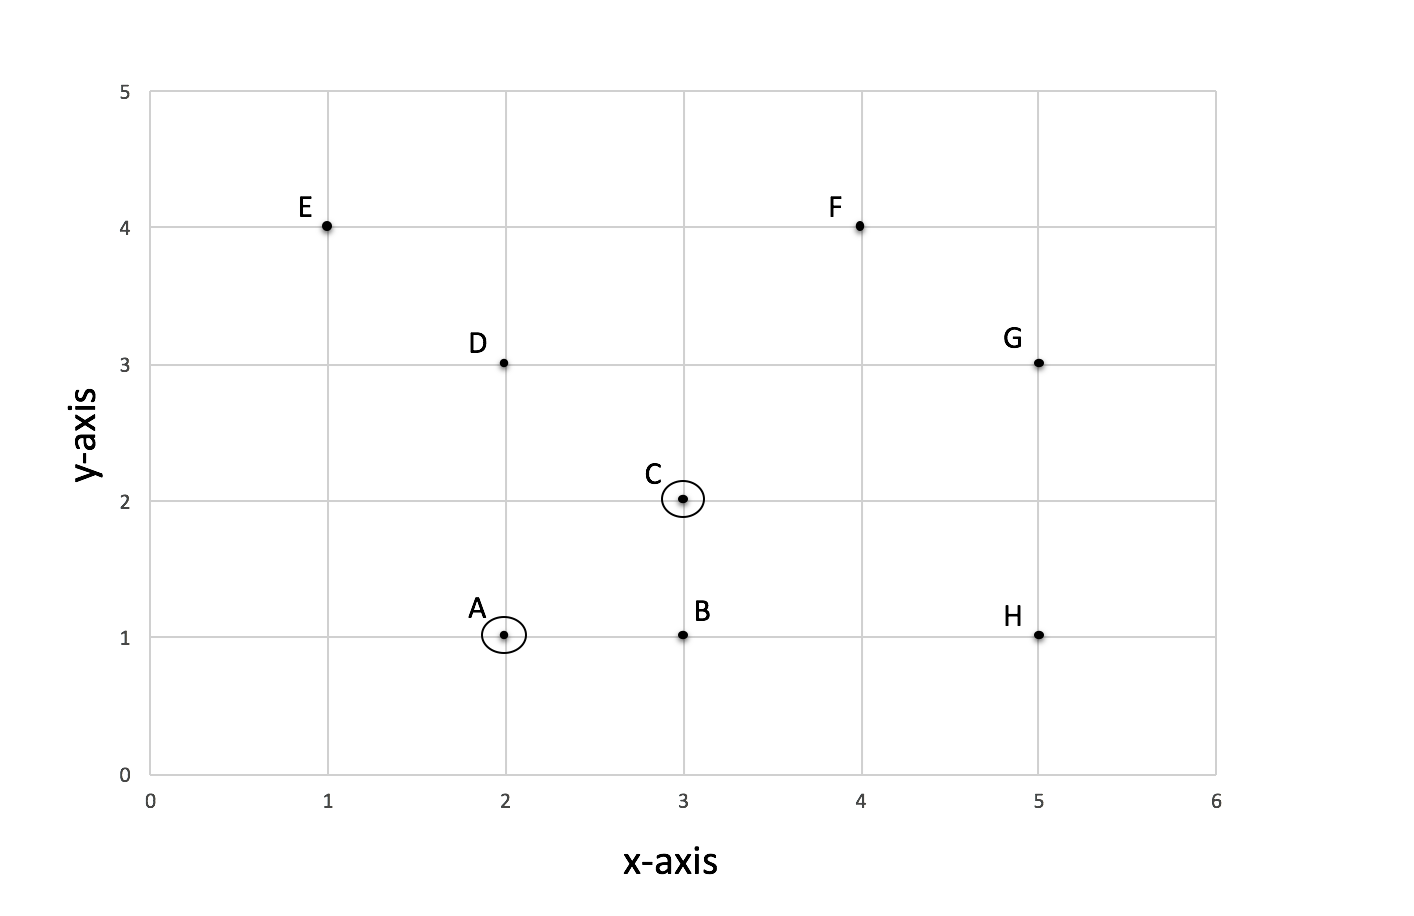
\includegraphics[width=0.8\linewidth]{figures/k-cluster.jpg}
			\caption{k-clustering algorithm}
			\end{figure}
\end{frame}

\begin{frame}{K-Clustering}
  Examples of Conflict in vertex related problems.\\
  1) K-Cluster Algorithm\\
  A=(2,1), B=(3,1), C=(3,2), D=(2,3),\\
  E=(1,4), F=(4,4), G=(5,3), H=(5,1)\\ where $B, D, E, F, G, H$ are objects\\
  $A$ and $C$ are two clusters.\\
\end{frame}

\begin{frame}{K-clustering}
  Calculating Euclidean distance from each object to both of the clusters:\\
  $DA$=$\sqrt{{(2-2)}^2+{(3-1)}^2}=2$,
  $DC$=$\sqrt{{(2-3)}^2+{(3-2)}^2}=\sqrt{2}$\\
  $\therefore DC<DA$\\
  $BA$ = $\sqrt{{(3-2)}^2+{(1-1)}^2}=1$,
  $BC$ = $\sqrt{{(3-3)}^2+{(2-1)}^2}=1$\\
  $\therefore AB=BC$\\
  $AE$=$\sqrt{{(2-1)}^2+{(1-4)}^2}=\sqrt{10}$,
  $CE$=$\sqrt{{(3-1)}^2+{(2-4)}^2}=\sqrt{8}$\\
  $\therefore CE<AE$\\
\end{frame}

\begin{frame}{K-Clustering}
  $AF$=$\sqrt{{(4-2)}^2+{(4-1)}^2}=\sqrt{13}$,
  $CF$=$\sqrt{{(4-3)}^2+{(4-2)}^2}=\sqrt{5}$\\
  $\therefore CF<AF$\\
  $AG$=$\sqrt{{(5-2)}^2+{(3-1)}^2}=\sqrt{13}$,
  $CG$=$\sqrt{{(5-3)}^2+{(3-2)}^2}=\sqrt{5}$\\
  $\therefore CG<AG$\\
  $AH$=$\sqrt{{(5-2)}^2+{(1-1)}^2}=3$,
  $CH$=$\sqrt{{(5-3)}^2+{(1-2)}^2}=\sqrt{5}$\\
  $\therefore AH<CH$\\
\end{frame}

  \section{Solution}
\subsection{Naive Priority}

\begin{frame}{Naive Priority}
  \begin{itemize}
    \item Assign priority to conflicting requests
    \item User needs to specify the order to provide deterministic results and resolve concurrent conflict
    \item Challenge: Naive scheme that assumes user can predict all possible combination that may happen for specific application
  \end{itemize}
  \end{frame}

\begin{frame}{Vertex Inclusion}
	Conflict in K-cluster
			\begin{figure}
			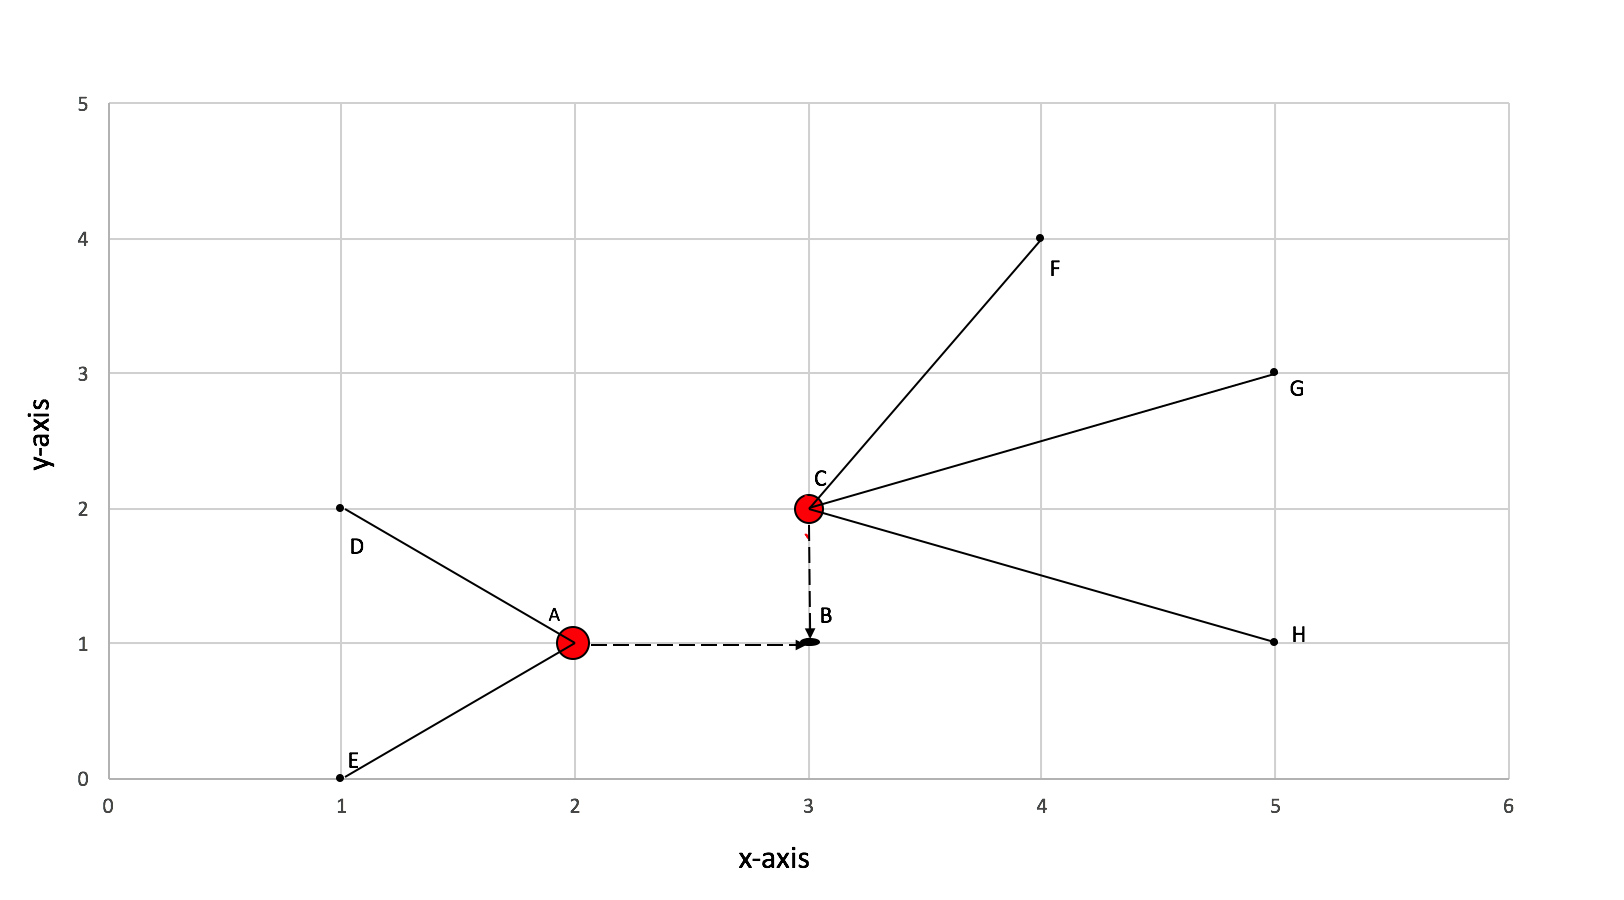
\includegraphics[width=0.6\linewidth]{figures/priority2.png}
			\caption{Solution Using Priority Models}
			\end{figure}
\end{frame}

\begin{frame}{Vertex addition}
	Conflict in vertex addition
			\begin{figure}
			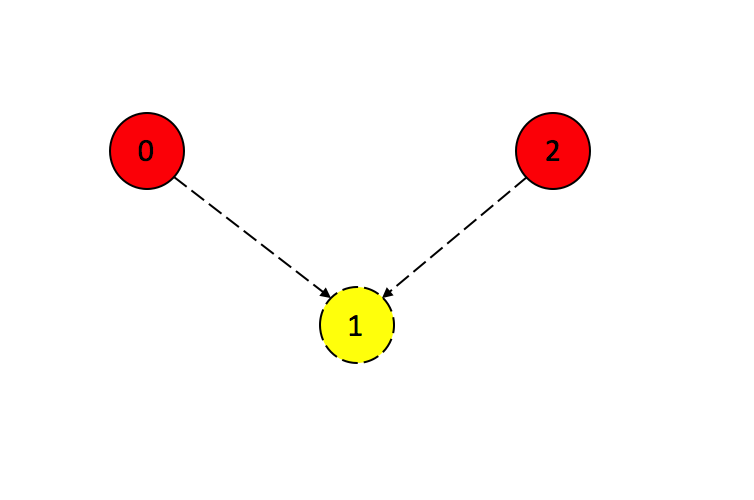
\includegraphics[width=0.6\linewidth]{figures/priority1.png}
			\caption{Solution Using Priority Models}
			\end{figure}
\end{frame}

\subsection{Consistency Models}
\begin{frame}{K-Clustering}
	Conflict in k-clustering algorithm
			\begin{figure}
			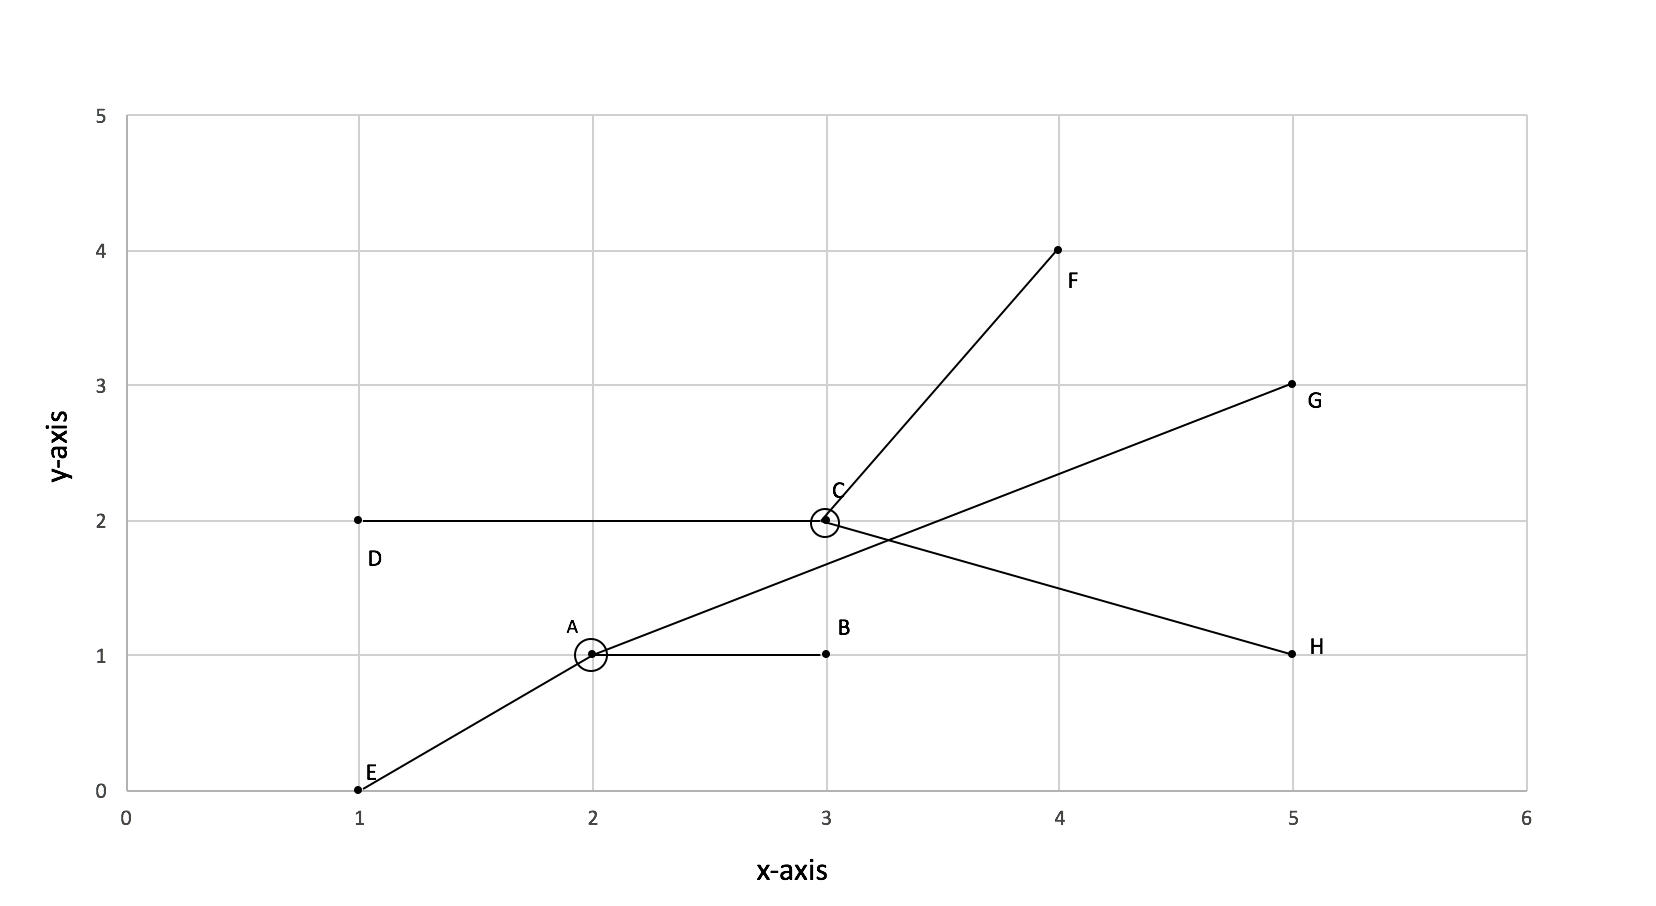
\includegraphics[width=0.8\linewidth]{figures/kcluster1.jpg}
			\caption{Solution Using Consistency Models}
			\end{figure}
\end{frame}

\begin{frame}{K-Clustering}
  Calculating Euclidean distance from each object to both of the clusters:\\
  $DA$=$\sqrt{{(1-2)}^2+{(2-1)}^2}=\sqrt{2}$,
  $DC$=$\sqrt{{(1-3)}^2+{(2-2)}^2}=2$\\
  $\therefore DA<DC$\\
  $BA$ = $\sqrt{{(3-2)}^2+{(1-1)}^2}=1$,
  $BC$ = $\sqrt{{(3-3)}^2+{(2-1)}^2}=1$\\
  $\therefore BA=BC$\\
  $EA$=$\sqrt{{(2-1)}^2+{(1-0)}^2}=\sqrt{2}$,
  $EC$=$\sqrt{{(3-1)}^2+{(2-0)}^2}=\sqrt{8}$\\
  $\therefore EA<EC$\\
\end{frame}

\begin{frame}{K-Clustering}
  $FA$=$\sqrt{{(4-2)}^2+{(4-1)}^2}=\sqrt{13}$,
  $FC$=$\sqrt{{(4-3)}^2+{(4-2)}^2}=\sqrt{5}$\\
  $\therefore FC<FA$\\
  $GA$=$\sqrt{{(5-2)}^2+{(3-1)}^2}=\sqrt{13}$,$GC$=$\sqrt{{(5-3)}^2+{(3-2)}^2}=\sqrt{5}$\\
  $\therefore GC<GA$\\
  $HA$=$\sqrt{{(5-2)}^2+{(1-1)}^2}=3$,
  $HC$=$\sqrt{{(5-3)}^2+{(1-2)}^2}=\sqrt{5}$\\
  $\therefore HC<HA$\\
\end{frame}

\begin{frame}{K-Clustering}
	Conflict in k-clustering algorithm
			\begin{figure}
			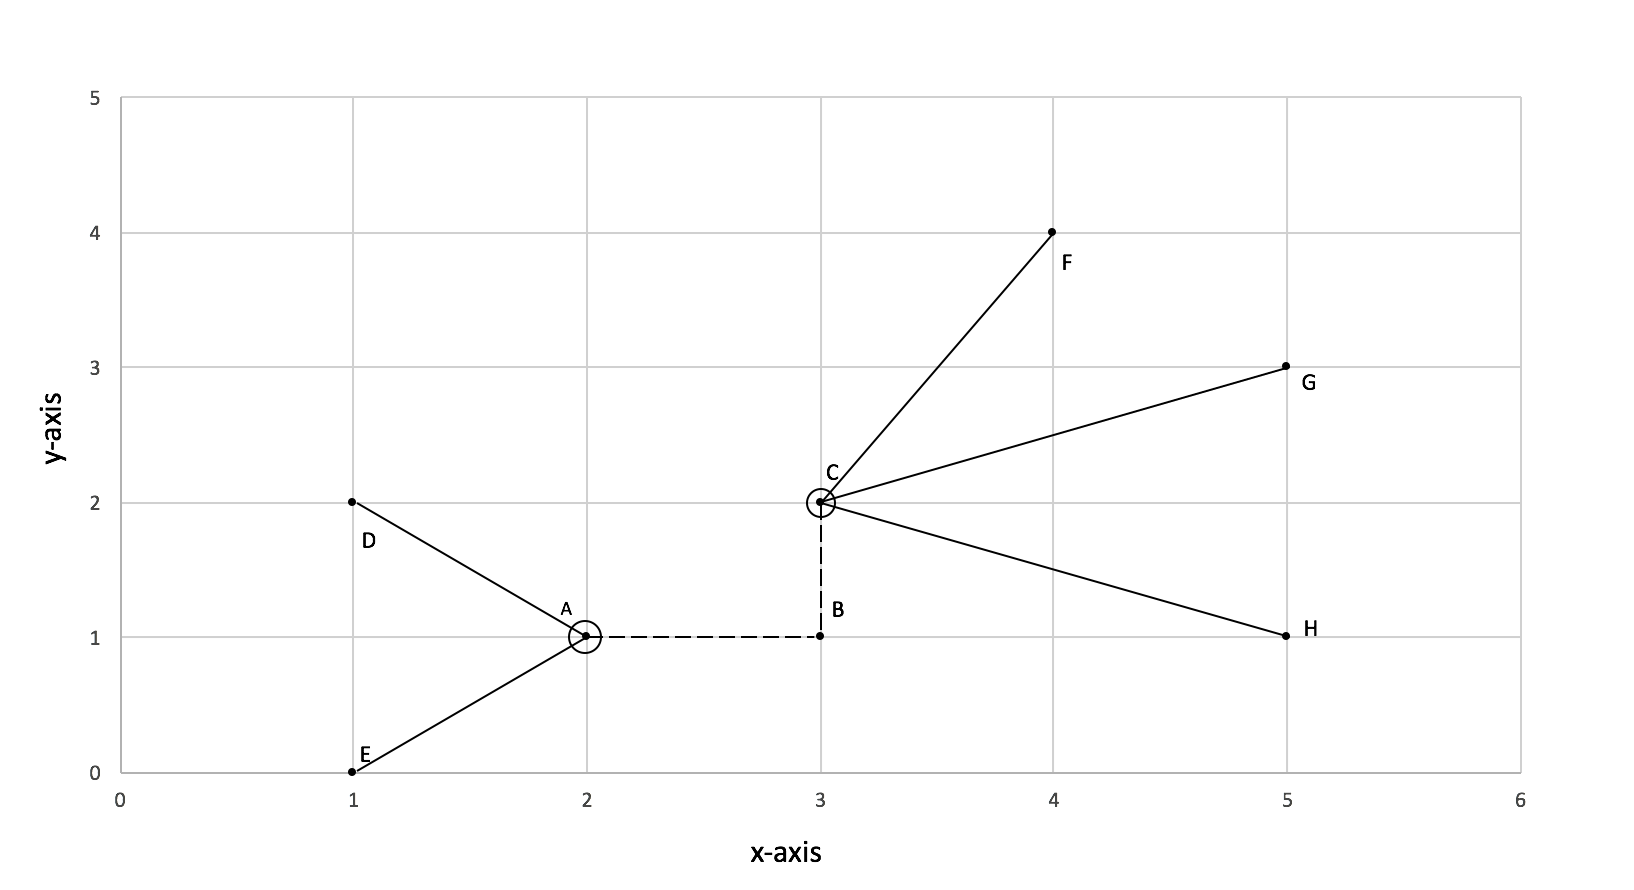
\includegraphics[width=0.8\linewidth]{figures/kcluster2.jpg}
			\caption{Solution Using Consistency Models}
			\end{figure}
\end{frame}

\begin{frame}{K-Clustering}
	Conflict in k-clustering algorithm
			\begin{figure}
			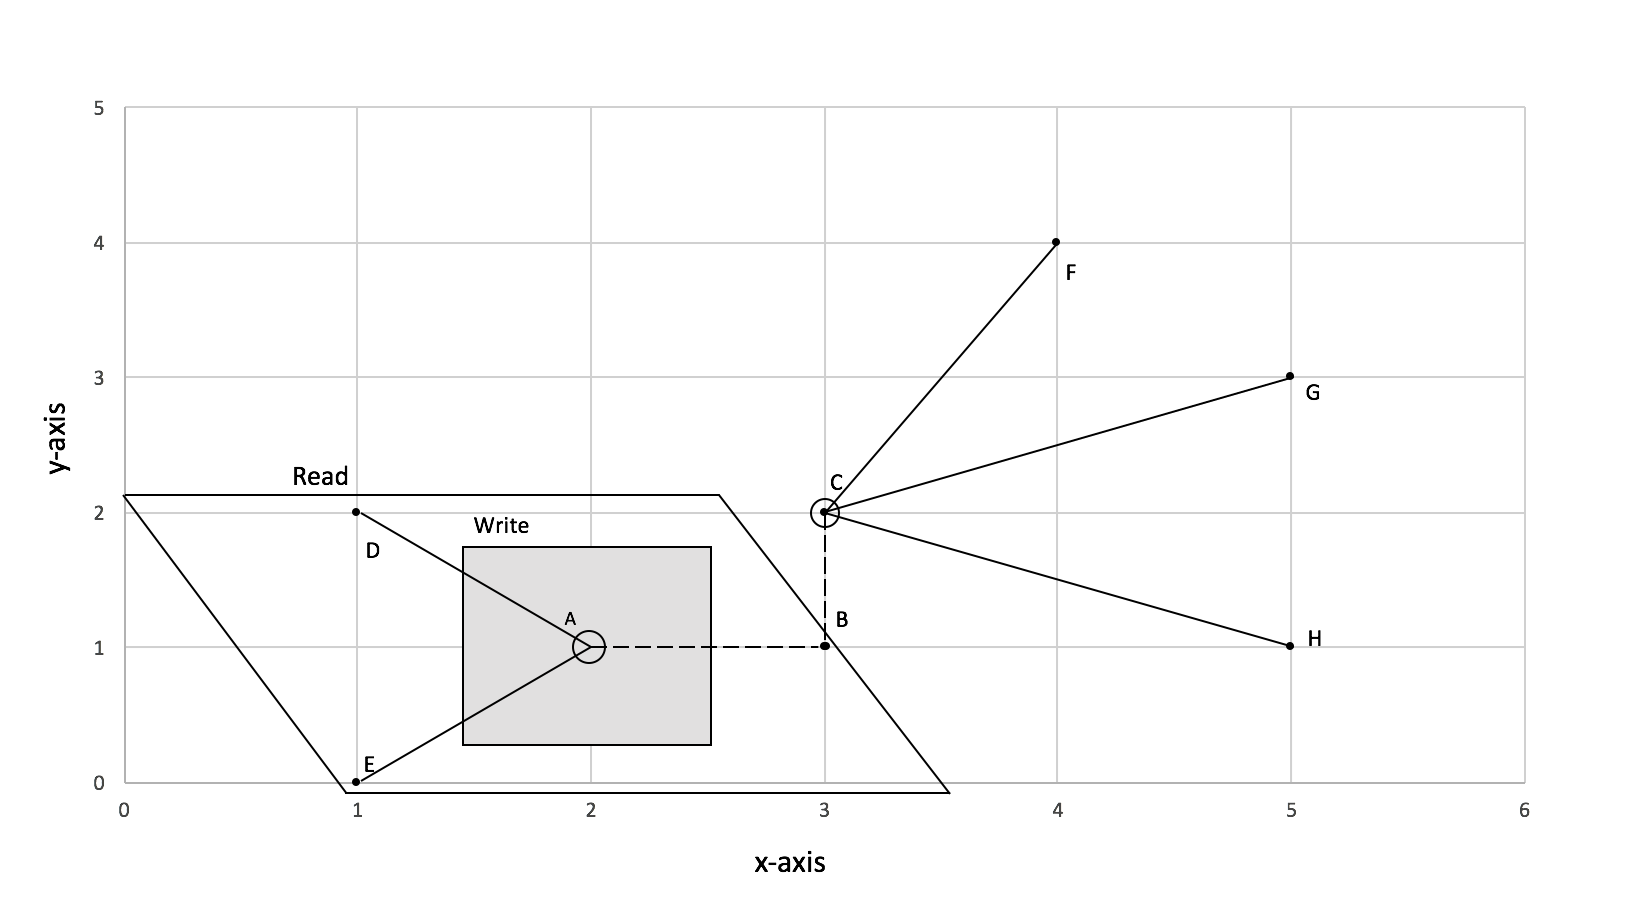
\includegraphics[width=0.8\linewidth]{figures/kcluster3.png}
			\caption{Solution Using Consistency Models}
			\end{figure}
\end{frame}


\begin{frame}{Vertex addition}
	Conflict in vertex addition
			\begin{figure}
			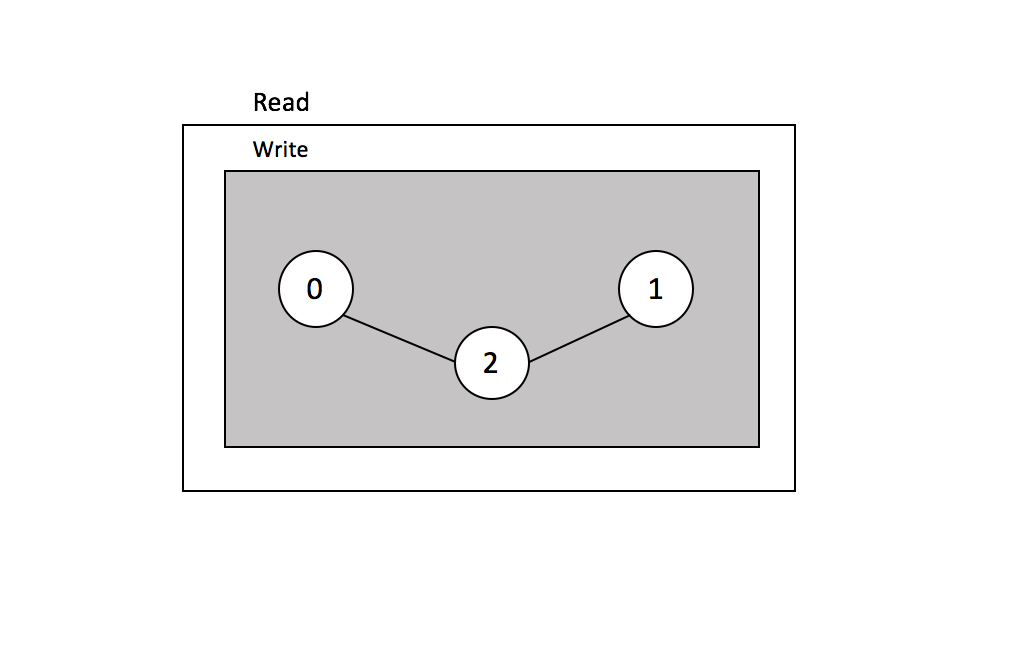
\includegraphics[width=0.6\linewidth]{figures/vnode1.png}
			\caption{Solution Using Consistency Models}
			\end{figure}
\end{frame}

  
\subsection{Graph Specification}
\begin{frame}{Graph Specifications}
% Abstract Refinement Types, Vazou \textit{et al.}, ESOP '13.

Check properties of the vertices and edges affected by the mutation against
defined specifications, for example:

\begin{figure}
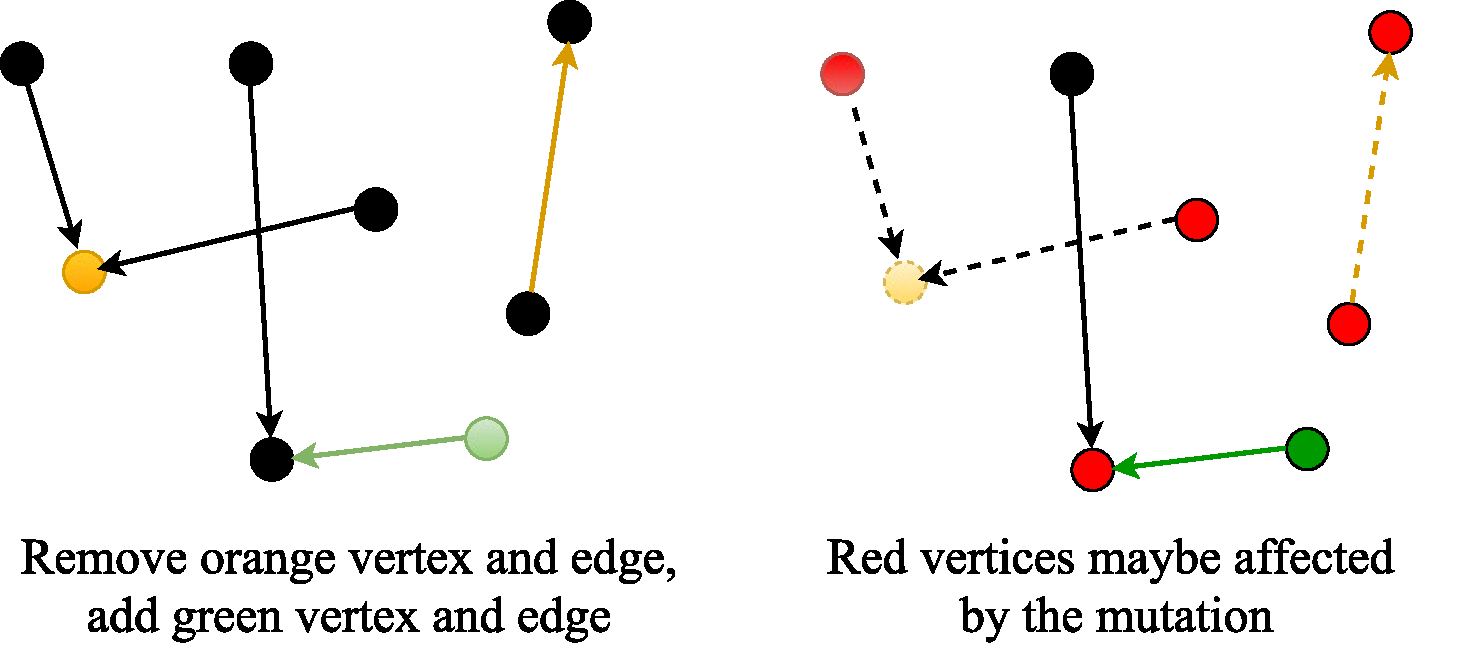
\includegraphics[width=0.7\linewidth]{figures/fig-specification1.pdf}
\end{figure}

Use assertions to check the correctness of mutations

\begin{itemize}
  \item Maximum in-degree < 2
\end{itemize}

\end{frame}


\begin{frame}
K-clustering problem:
\begin{itemize}
  \item Maximum of 1 cluster node connected
\end{itemize}

Restrictions:\\
  Lack of global information, specification may not be able to be on the
  global level

  e.g. checking that the edges being added indeed minimizes the Euclidean
  distance may not be possible as it needs information from different vertices
\end{frame}

% \begin{frame}
% \begin{figure}
% 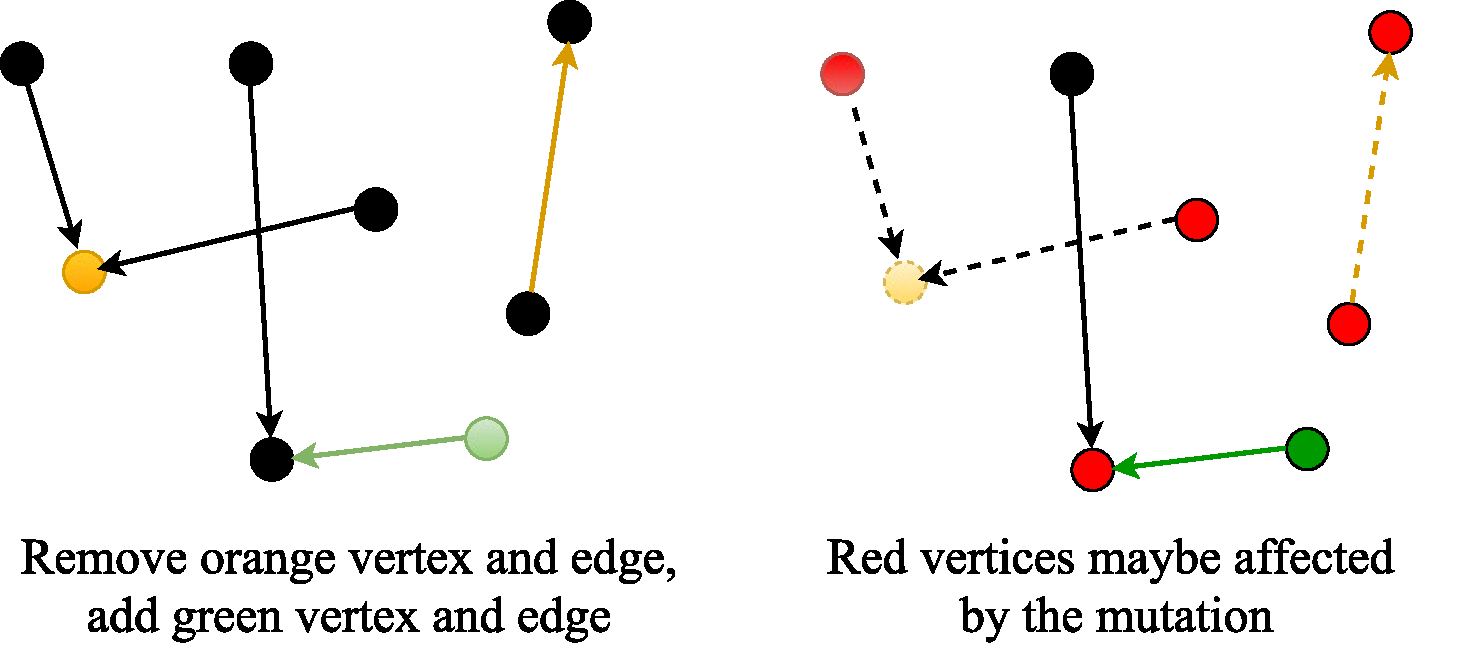
\includegraphics[width=0.8\linewidth]{figures/fig-specification1.pdf}
% \end{figure}
% \end{frame}

  \section{Formalization}
\begin{frame}{Semantics}
\textbf{Definition 1.} A directed graph is a tuple $G = (V, E)$ where V is a
finite set of vertices, i.e., $V={v_1,\ldots,v_n}$, and E is a finite set of
directed edges which are ordered pairs of V, i.e.,
$E={e_{1},\ldots,e_{m}}\subseteq V\times V$, where each $e_{i}=(v_{j},v_{k})$
for some j, k.
\end{frame}

\begin{frame}
Graph mutation semantics:\\
\begin{large}
(Edge\_Insertion)\\
\end{large}
\hspace{3cm}
\begin{Large}
$\frac{v_{j}\in V, v_{k}\in V}{(v_{j},v_{k})i_{e}:G(V,E)\rightarrow (V,E\cup
\{v_{i},v_{k}\})}$
\end{Large}

\vspace{5mm}

\begin{large}
(Edge\_Removal)\\
\end{large}
\hspace{3cm}
\begin{Large}
$\frac{v_{j}\in V, v_{k}\in V}{(v_{j},v_{k})r_e:G(V,E)\rightarrow
(V,E\setminus \{v_{i},v_{k}\})}$\\
\end{Large}
\vspace{5mm}
\begin{large}
(Vertex\_Insertion)\\
\end{large}
\hspace{3cm}
\begin{Large}
$\frac{v\notin V}{(v)i_v:G(V,E)\rightarrow
(V\cup v,E\})}$\\
\end{Large}
\vspace{5mm}
\begin{large}
(Vertex\_Removal)\\
\end{large}
\hspace{3cm}
\begin{Large}
$\frac{v\in V, E' = \{(v_j, v_k)\in E, v_j=v \lor v_k=v\}
}{(v)i_r:G(V,E)\rightarrow (V\cup v,E\setminus E' \})}$
\end{Large}

\end{frame}

\begin{frame}
Local semantics:\\
\begin{itemize}
  \item The four operations as expressions.
  \item Evaluate the four mutation expressions by pushing it into a global
  expression queue.
\end{itemize}

Global semantics:\\
\begin{itemize}
  \item Evaluate processes one by one until all processes reach barrier state.
  \item Mutate the global graph using the graph mutation requests using the
  global expression queue and the graph mutation semantics.
  \item Given a graph and a mutation request queue, the mutation is invalid, if:
  \begin{itemize}
    \item Output is not a well-formed graph
    \item Output graph does not have the graph properties the
    provided specification specifies.
  \end{itemize}
\end{itemize}


\end{frame}




  \section{Related Works}

\begin{frame}{Reference(s):}
\begin{itemize}
 \item Yucheng Low, Joseph Gonzalez, Aapo Kyrola, Danny Bickson, Carlos Guestrin, and Joseph M. Hellerstein, "GraphLab: A New Parallel Framework for Machine Learning, In Uncertainty in Artificial Intelligence, 2010.
\item Refinement type reference?
\item Grzegorz Malewicz, Matthew H. Austern, Aart J. C. Bik, James C. Dehnert, Ilan Horn,
Naty Leiser, and Grzegorz Czajkowski, "Pregel: A System for Large-Scale Graph Processing", SIGMOD, 2010.
    \end{itemize}
\end{frame}


\begin{frame}{Reference(s):}
\begin{itemize}
\item Semih Salihoglu and Jennifer Widom, "GPS: A Graph Processing System", Proc. International Conference on Scientific and Statistical Database Management (SSDBM), 2013.
\item Serafettin Tasci and Murat Demirbas, "Giraphx: Parallel Yet Serializable Large-Scale Graph Processing", EuroPar, 2013. 
\item Joseph E. Gonzalez, Yucheng Low, Haijie Gu, Danny Bickson, Carlos Guestrin, "PowerGraph: Distributed Graph-Parallel Computation on Natural Graphs", OSDI, 2012.     
    \end{itemize}
\end{frame}
 

  \begin{frame}
\begin{beamercolorbox}[center]{white}
  {\Large Questions?}

  \vspace{2em}\hfill

  \url{http://www.cs.iastate.edu/~WEBSITE/}
\end{beamercolorbox}
\end{frame}

\end{document}
